%% Bemærk:
%%          Resten af rapporten følger en stil hvor indledninger skrives
%%          med \sffamlily-typen. Denne stil bør også følges her.
%%
{\sffamily
I vores program er der fire forskellige tærskelværdier som påvirker
hvordan maleriet analyseres, nå regioner udtrækning af maleriet.
Margionbredde, kandtdetektion, flootfill og sløring. I dette sektion vil
vi finde værdier for de fire tærskelværdier, samt forklaring hvorfor vi
har valt lige de tal. Malerierne som er brugt i afprøvning er specielt
udvalgt for deres illustrative aspekt. 
}

\subsection{Størrelsen på margin}
Vi regner marginbredde ud fra en procent stats, som vi kalder $\psi$, af
billedets $B$ og $H$. I defination \ref{margin_min} definere vi den
minimale størrelse på margin til $2.1 \%$. Så $\psi$ skal være støre en
$2.1 \%$. 

I defination \ref{margin_max}
Den minimale forskel på to snit vi foretager os, er forskellen mellem
det gyldne snit og $\frac{2}{3}$. I definition \ref{margin_max} er den
maksimale bredde margin kan have $2.43\%$. For at marginen ikke
overlapper. Så $\psi$ skal være mindre en $2.43\%$. 

Det vil sige at $\psi \in [2.1, 2.43]$. Vi har valt at
sætte $\psi = 2.4$, da vi derved kan tage højde for uforresette
usikkerhed.

\subsection{Afvigelsen af farver i kandtdetection}
Vi bruger kandtdetection til, er af finde en kanter rundt om de regioner
som vi mener er interessante, og undgå de kanter som ligger inde i
regioner. Begge de 2 mål kan ikke altid opfyldes, men vi kan komme så
tæt på et krompromi mellem en perfekt kant rund om region og ingen
kanter inde i region som mulige. Dette gøres ved at ændre 2
tærskelværdier i kantdetectionen. Vi har valt at dele billederne som vi
observere op i 9 kategorier, se tabel \ref{thressholdsTabelKant},
Kategorier er en grove opdeling af billederne efter detaljer og farve
intensitet, som bruges til at give en bedre indblik på billedets
opbygning. 

\subsubsection{Sammenligninger}
Vi har set på 9 malerier og har fundet de tærskelværdier som vi mener
passer bæst på malerierne. Vi vil illustrerer hvordan vi har fastsat
tærskelværdierne på maleriet \ref{kDetalier}.

Maleriet er malet med mange farver og med masser af detaljer. Vi ser
først på tærskelværdierne $(0,0),(100,100).....(600,600),(700,700)$ se
figur \ref{allesammen1} og \ref{allesammen2}, og finde det interval hvor
malerriet ikke har mistet nogle af kanterne rundt om regionerne endnu,
men vil det, i næste interval. I illustration vurdere vi det til
billedet \ref{300-300}, da billedet \ref{400-400} har mistet for mange
af de kanter, som vi gerne vil beholde.

Ved at sætte en af tærskelværdierne op lidt af gangen, kan vi igen få en
række billeder at vælge imellem. Se sammenligningen i figur
\ref{allesammen3}. Man kan se at det begynder at være svær at skelne
figurene i \ref{300-850} og der er lidt for mange kanter i
\ref{300-700}.

Vi har valgt at fastsætte tærskeværdigerne til $(300,750)$. Det maleri
vi lige har brugt er ikke særlige repræsentativ for helle vores maleri
database. så vi har taget 8 andre billeder og brugt samme metode på dem og fastsat en
middel tærskelværdi. Vi viser her en lille udsnit af dem, se figur
\ref{en}, \ref{to} og \ref{tre}.
\clearpage
\begin{figure}[p]
    \centering
    \subfloat[(100,100)]{
        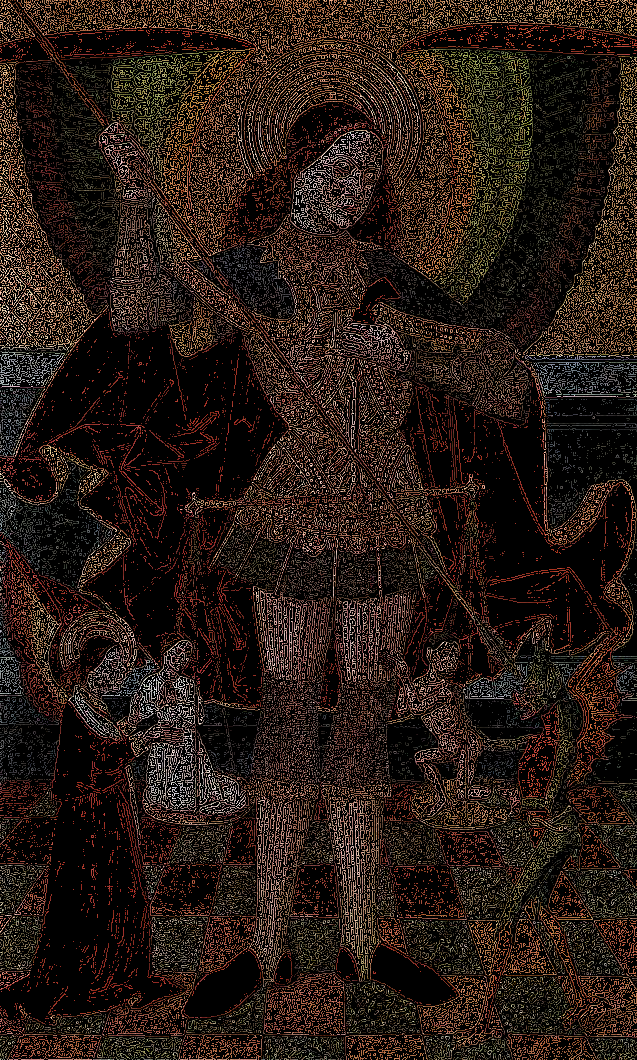
\includegraphics[angle=0,width=0.45\textwidth]{afsnit/afprovning/billeder/thressholds/krafitige_farver/krafite_detalier/1_iteration/100-100.png}
        \label{100-100}}\hspace{1em}
    \subfloat[(200,200)]{
        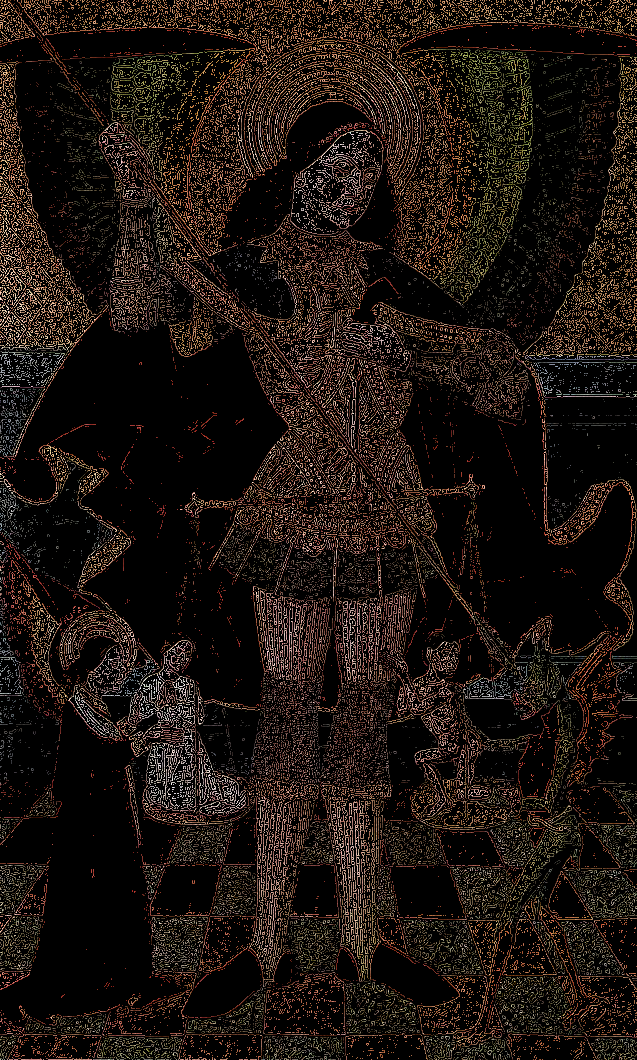
\includegraphics[angle=0,width=0.45\textwidth]{afsnit/afprovning/billeder/thressholds/krafitige_farver/krafite_detalier/1_iteration/200-200.png}
        \label{200-200}}\\
    \subfloat[(300,300)]{
        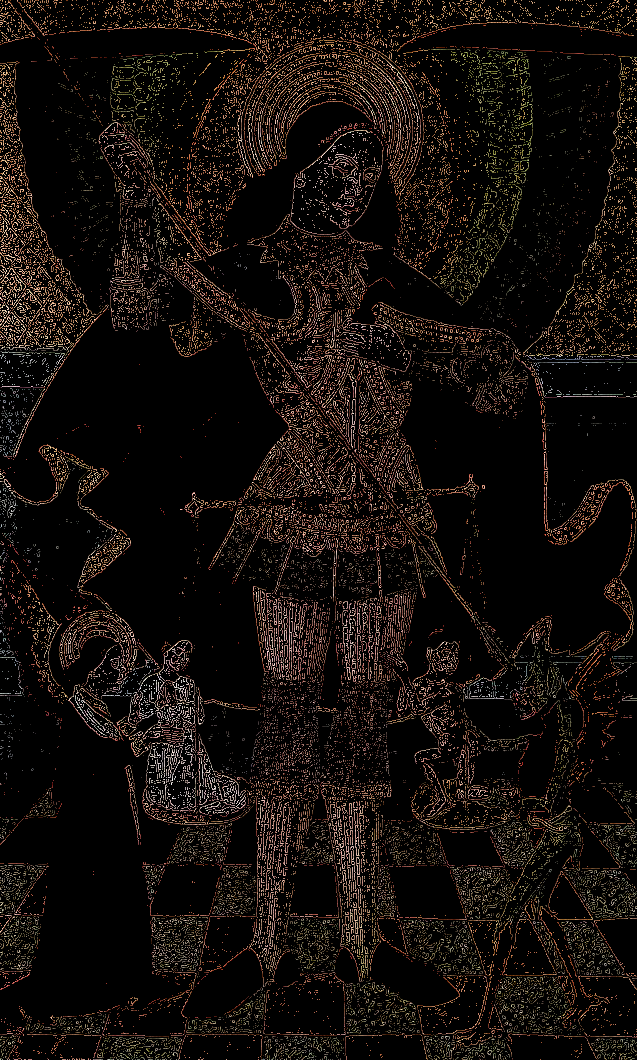
\includegraphics[angle=0,width=0.45\textwidth]{afsnit/afprovning/billeder/thressholds/krafitige_farver/krafite_detalier/1_iteration/300-300.png}
        \label{300-300}}\hspace{1em}
    \subfloat[(400,400)]{
        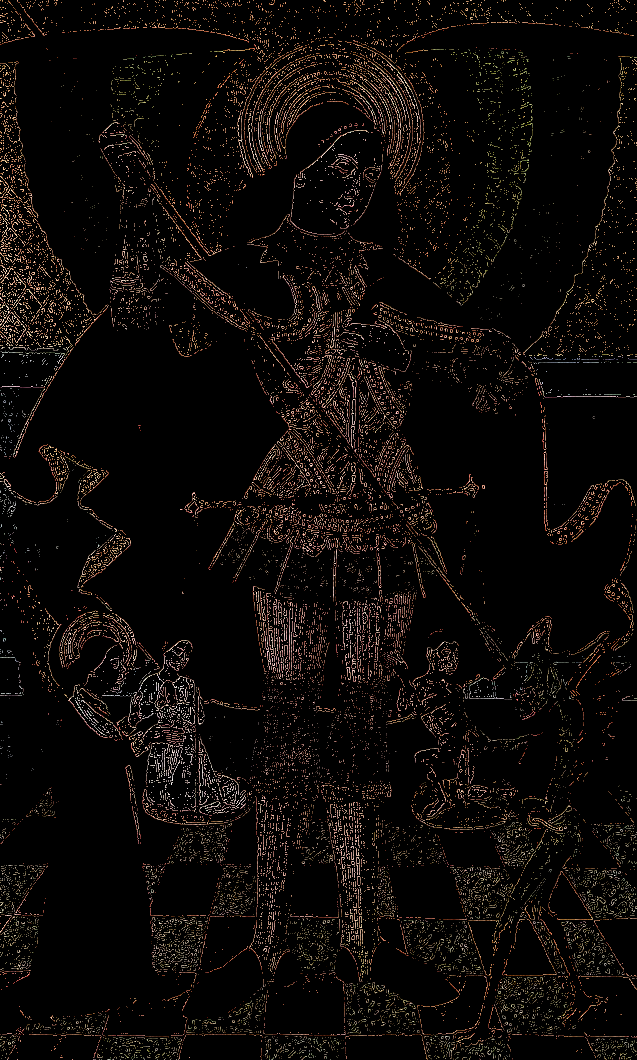
\includegraphics[angle=0,width=0.45\textwidth]{afsnit/afprovning/billeder/thressholds/krafitige_farver/krafite_detalier/1_iteration/400-400.png}
        \label{400-400}}
    \label{allesammen1}
    \caption{Edgedetection på maleriet \ref{kDetalier} som har mange detaliger og kraftige farver, med tærskelværdierne fra (100-100) til (400-400)}
\end{figure}

\clearpage

\begin{figure}[!h]
	\centering
	\subfloat[(500,500)]{
        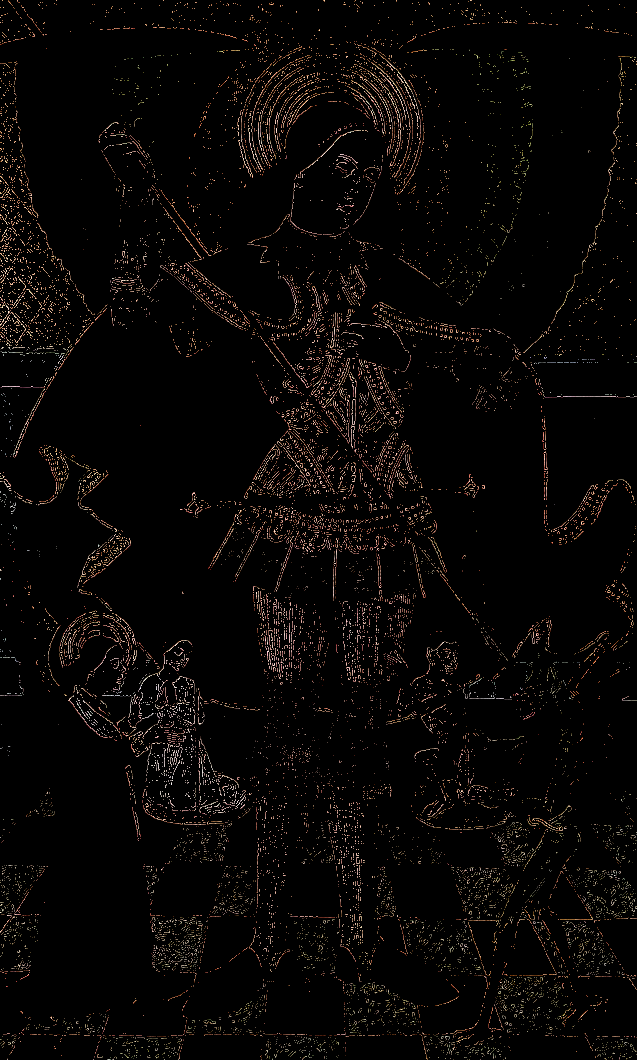
\includegraphics[angle=0,width=0.45\textwidth]{afsnit/afprovning/billeder/thressholds/krafitige_farver/krafite_detalier/1_iteration/500-500.png}
        \label{500-500}}\hspace{1em}
    \subfloat[(600,600)]{
        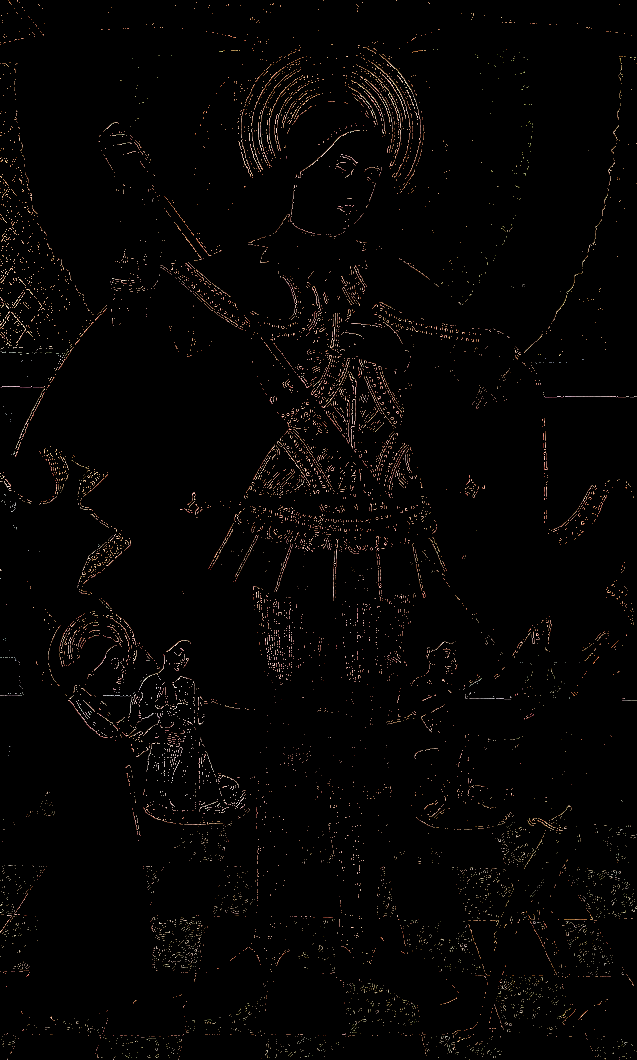
\includegraphics[angle=0,width=0.45\textwidth]{afsnit/afprovning/billeder/thressholds/krafitige_farver/krafite_detalier/1_iteration/600-600.png}
        \label{600-600}}\\
    \subfloat[(700,700)]{
        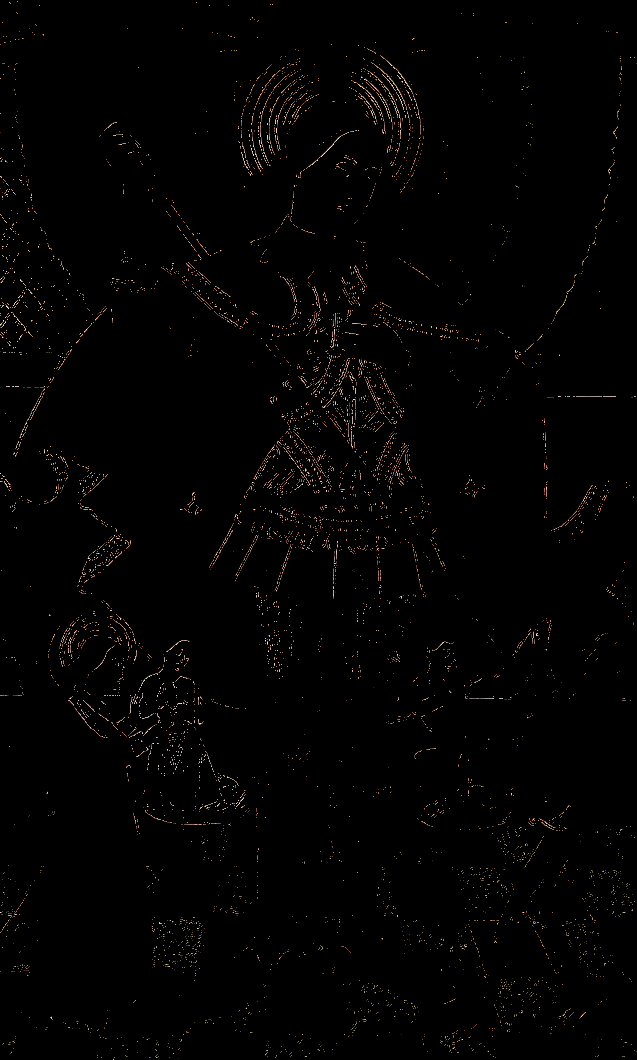
\includegraphics[angle=0,width=0.45\textwidth]{afsnit/afprovning/billeder/thressholds/krafitige_farver/krafite_detalier/1_iteration/700-700.png}
        \label{700-700}}\hspace{1em}
    \subfloat[Original. Navn: The Archangel Michae. År: Ca 1490 Af: Abadia, Juan de la]{
        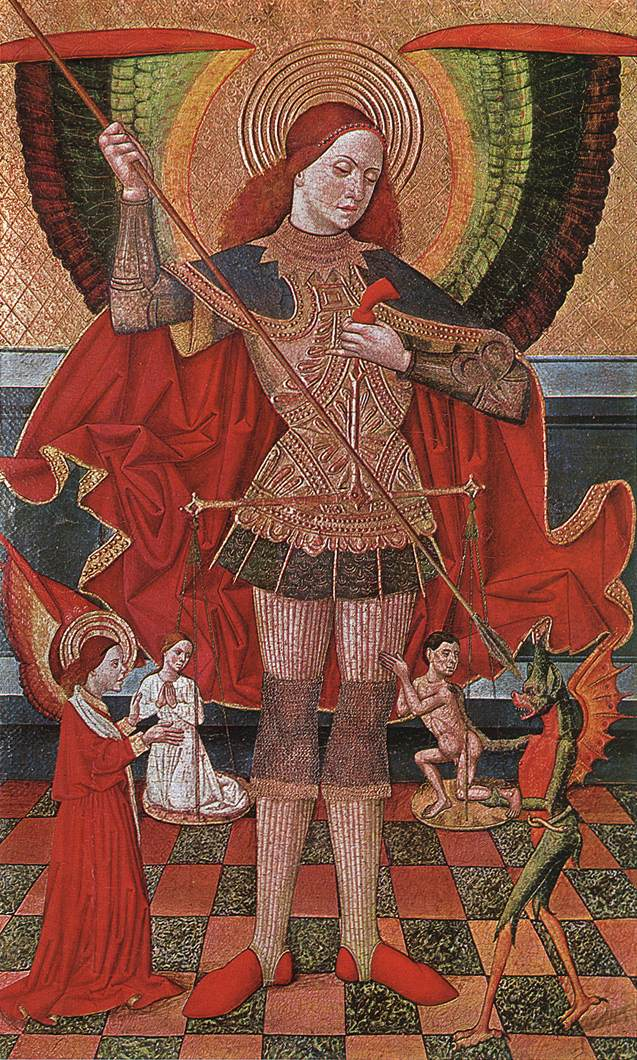
\includegraphics[angle=0,width=0.45\textwidth]{afsnit/afprovning/billeder/thressholds/krafitige_farver/krafite_detalier/kDetalier.jpg}
        \label{kDetalier}}
    \caption[]{Edgedetection på maleriet \ref{kDetalier} som har mange detaliger og kraftige farver, med tærskelværdierne fra (500-500) til (700-700)}
     \label{allesammen2}
\end{figure}

\begin{figure}[!h]
    \centering
    \subfloat[(300,700)]{
        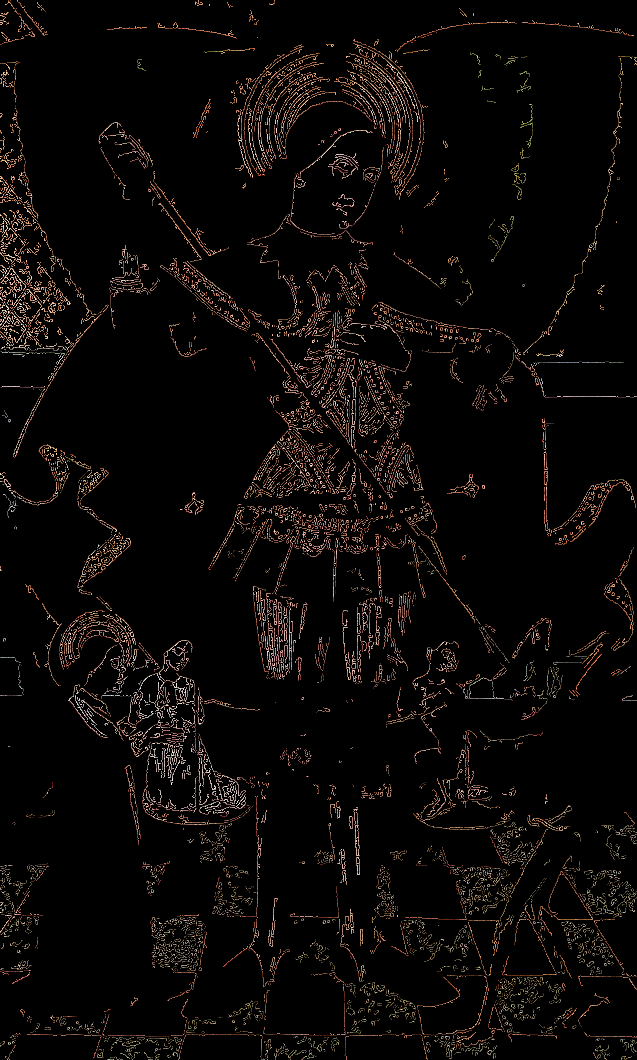
\includegraphics[angle=0,width=0.45\textwidth]{afsnit/afprovning/billeder/thressholds/krafitige_farver/krafite_detalier/2_iteration/300-700.png}
        \label{300-700}}\hspace{1em}
    \subfloat[(300,750)]{
        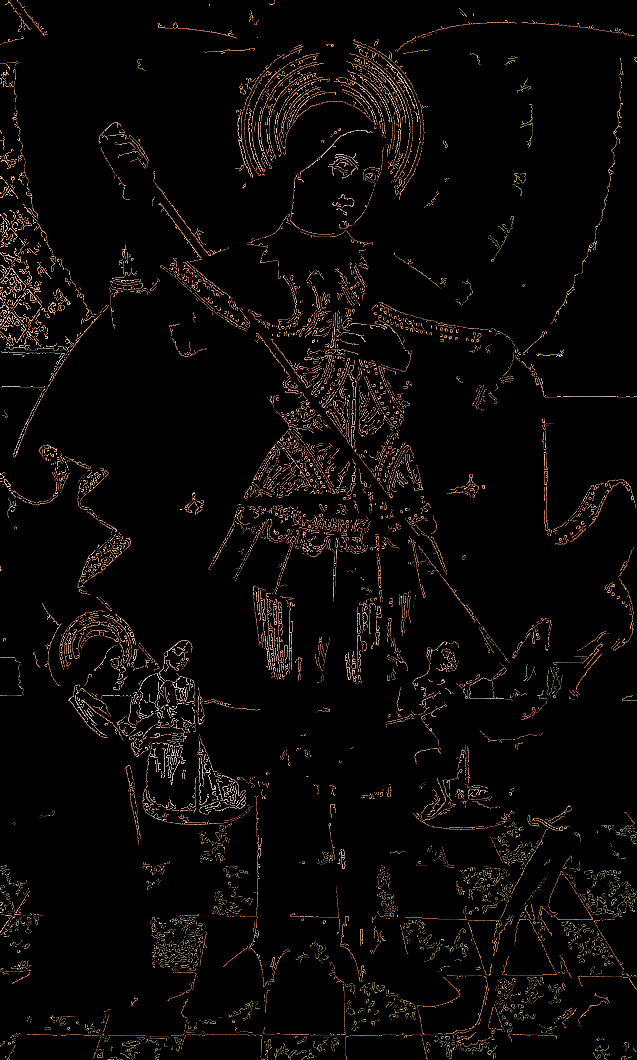
\includegraphics[angle=0,width=0.45\textwidth]{afsnit/afprovning/billeder/thressholds/krafitige_farver/krafite_detalier/2_iteration/300-750.png}
        \label{300-750}}\\
    \subfloat[(300,800)]{
        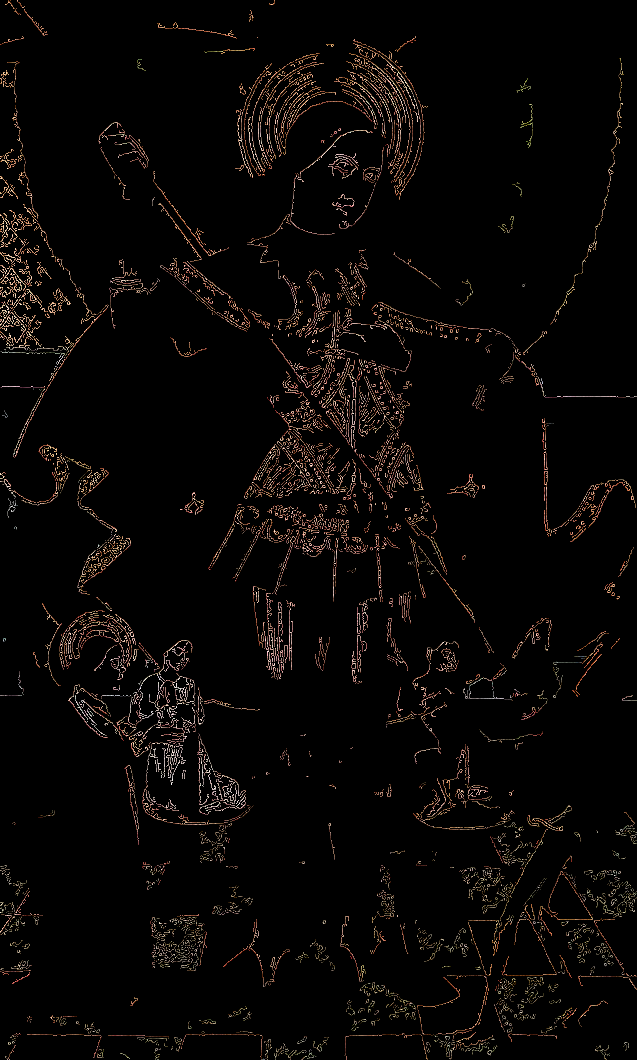
\includegraphics[angle=0,width=0.45\textwidth]{afsnit/afprovning/billeder/thressholds/krafitige_farver/krafite_detalier/2_iteration/300-800.png}
        \label{300-800}}\hspace{1em}
    \subfloat[(300,850)]{
        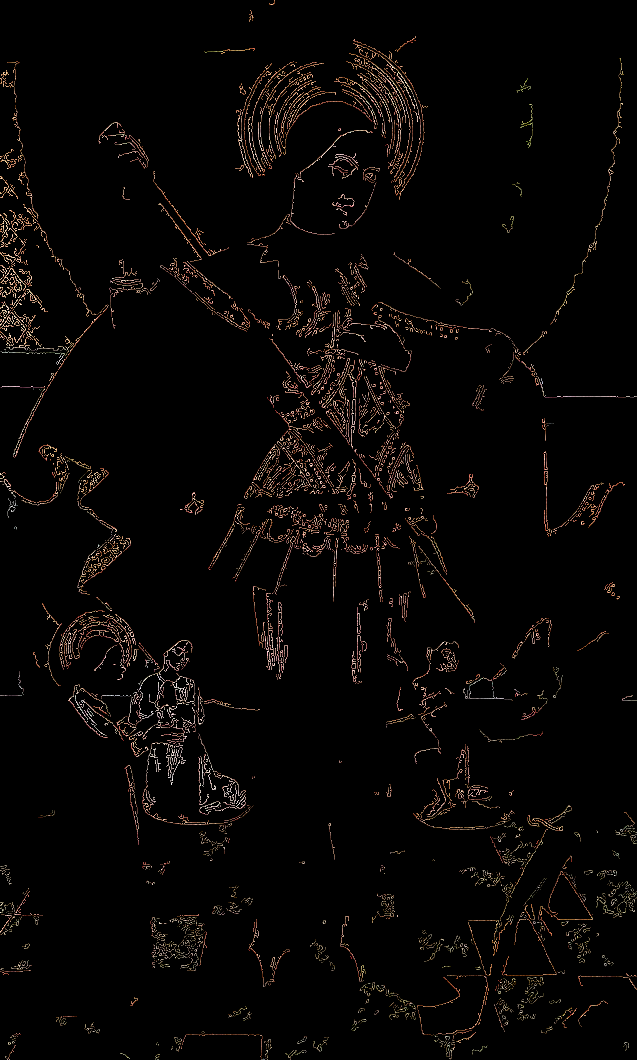
\includegraphics[angle=0,width=0.45\textwidth]{afsnit/afprovning/billeder/thressholds/krafitige_farver/krafite_detalier/2_iteration/300-850.png}
        \label{300-850}}
        \caption[]{Edgedetection hvor de 4 billeder som er intrasante taget med}
     \label{allesammen3}
\end{figure}
 
\begin{figure}[!h]
    \centering
    \subfloat[(100,250)]{
        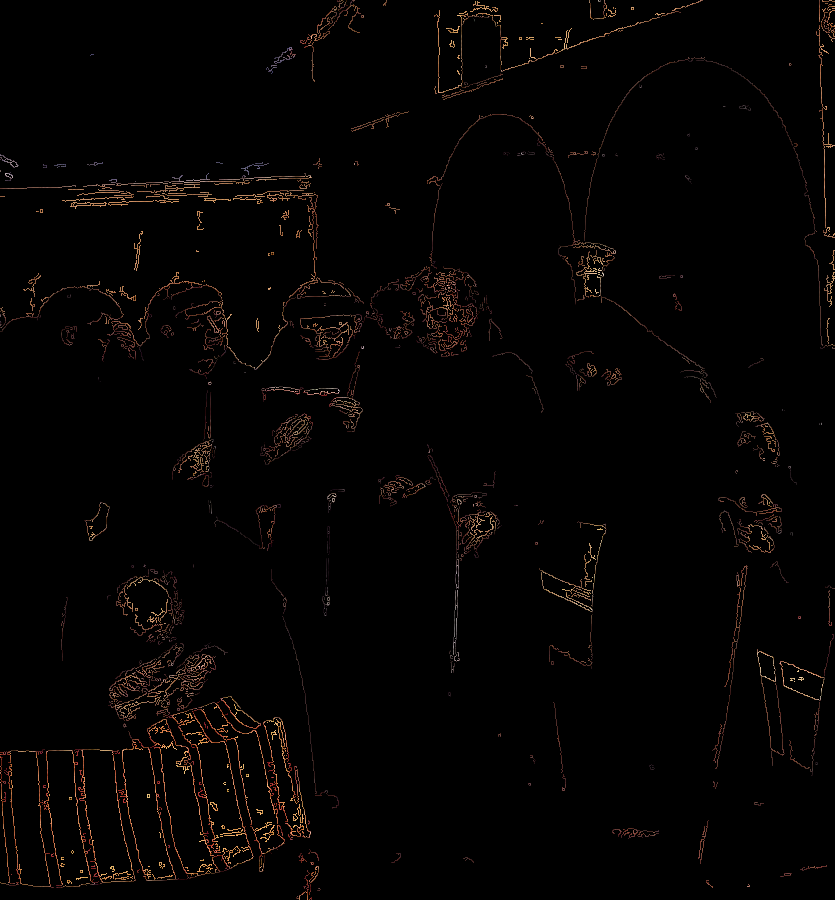
\includegraphics[angle=0,width=0.45\textwidth]{afsnit/afprovning/billeder/thressholds/svage_farver/svage_detalier/2_iteration/100-250.png}
        \label{100-250}}\hspace{1em}
    \subfloat[Orginal. Navn: The Lamentation over St Francis. År: 1440. Af: Angelico, Fra. ]{
        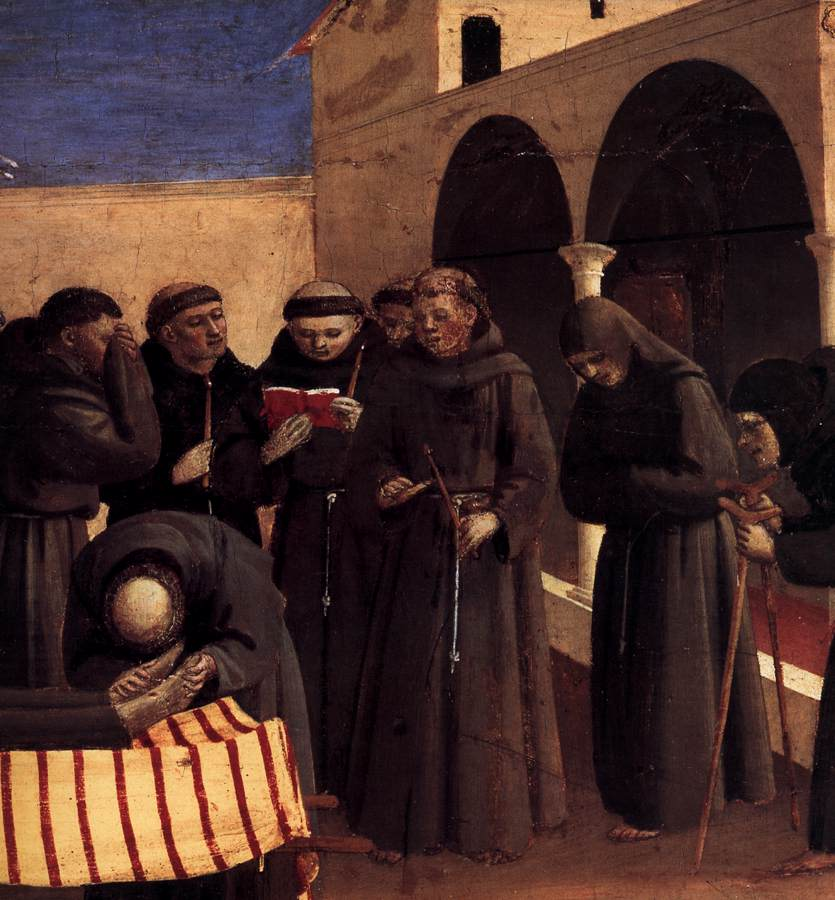
\includegraphics[angle=0,width=0.45\textwidth]{afsnit/afprovning/billeder/thressholds/svage_farver/svage_detalier/sDetalier.jpg}
        \label{Orginal1}}
        \caption[]{Edgedetection på et billedet med svage farver og få detalier, hvor tærskenværdigern [100,250] er den beste}
     \label{en}
\end{figure}

\begin{figure}[!h]
    \centering
    \subfloat[(100,240)]{
        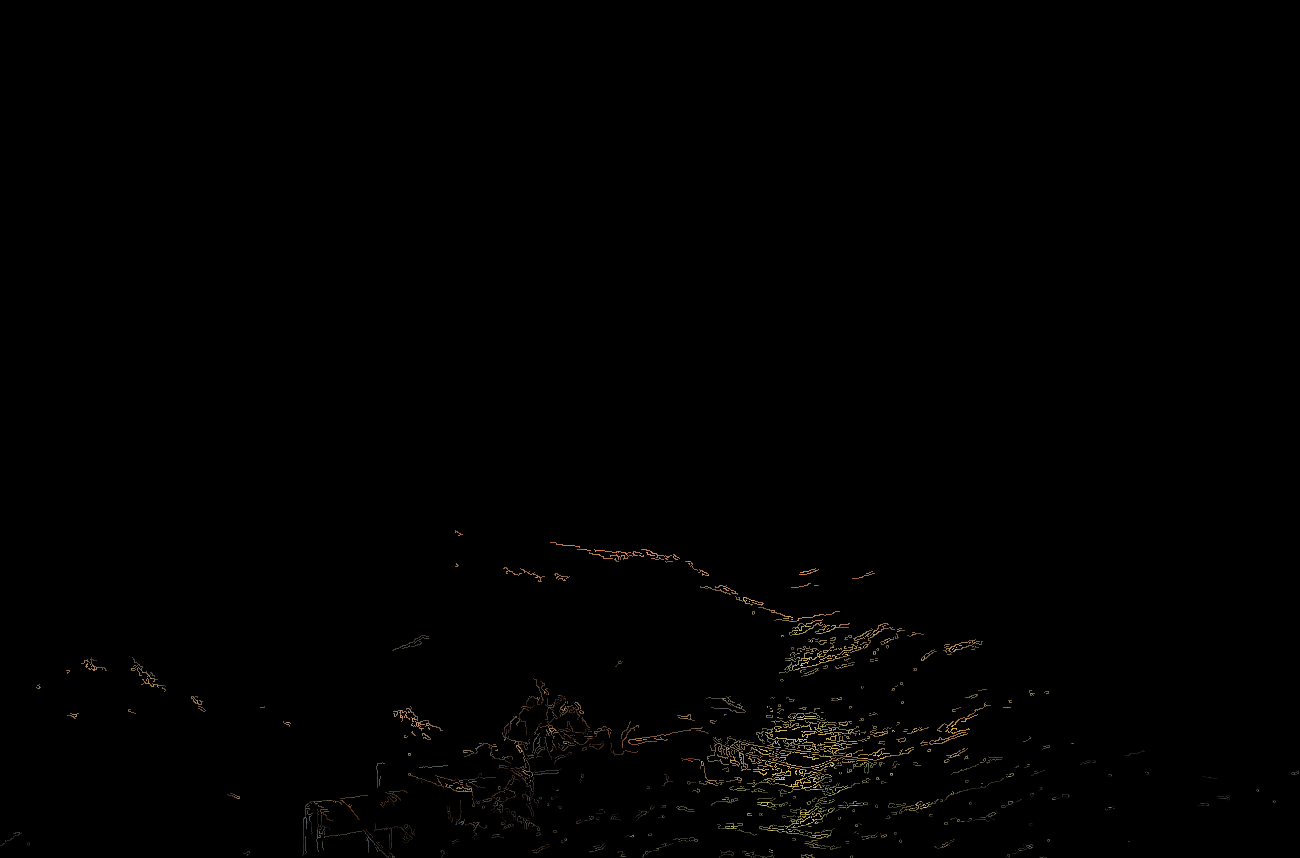
\includegraphics[angle=0,width=0.85\textwidth]{afsnit/afprovning/billeder/thressholds/medium_farver/svage_detalier/2_iteration/100-240.png}
        \label{100-240}}\\
    \subfloat[Orginal. Navn:The Ninth Wave. År:1850. Af:Aivazovsky, Ivan Konstantinovich.]{
        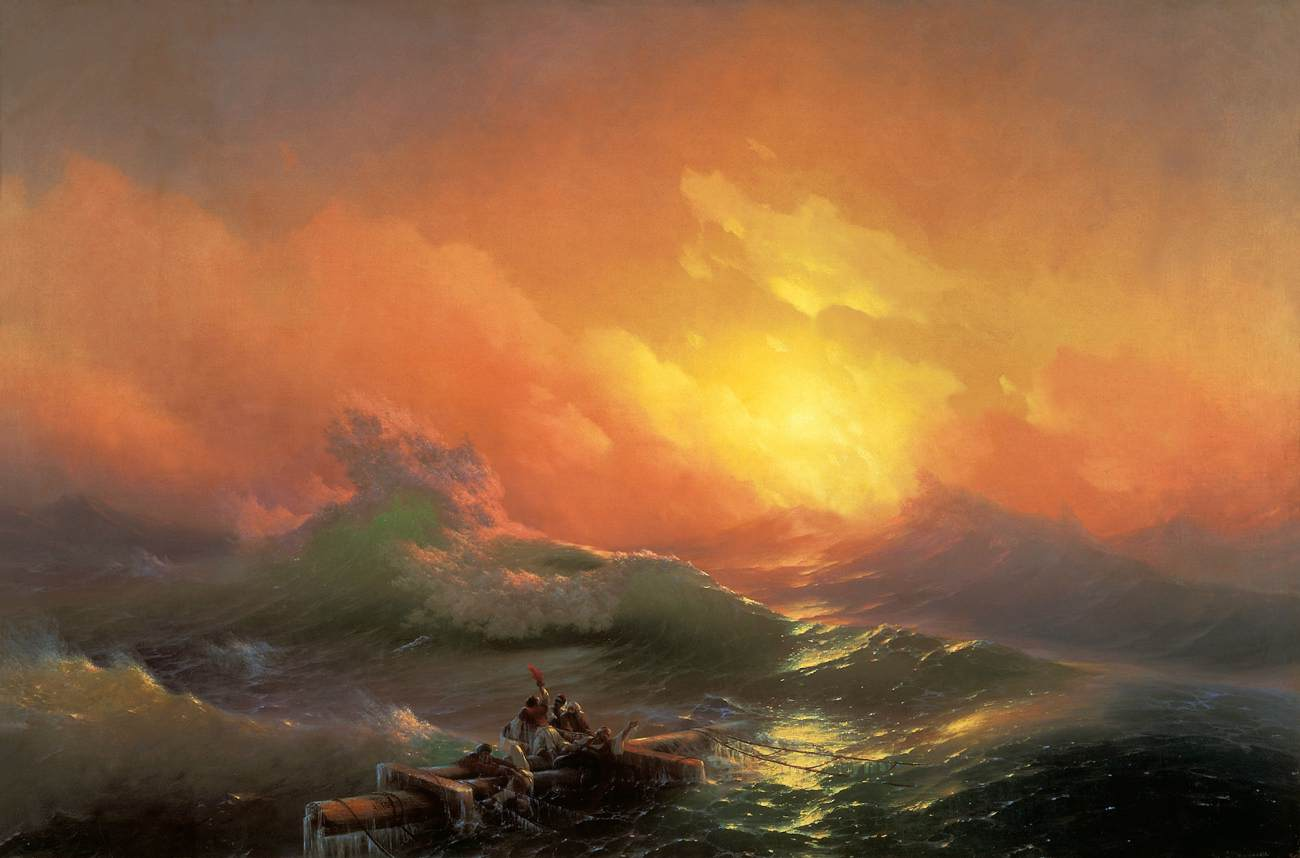
\includegraphics[angle=0,width=0.85\textwidth]{afsnit/afprovning/billeder/thressholds/medium_farver/svage_detalier/sDetalier1.jpg}
        \label{Orginal2}}
        \caption[]{Edgedetection på et billedet med medium farver og få detalier, hvor tærskenværdigern [100,240] er den beste}
     \label{to}
\end{figure}

\begin{figure}[!h]
    \centering
    \subfloat[(200,460)]{
        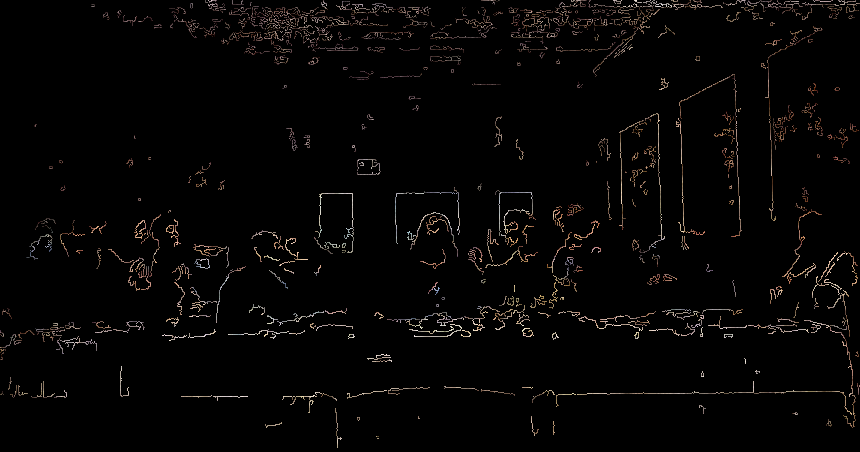
\includegraphics[angle=0,width=0.85\textwidth]{afsnit/afprovning/billeder/thressholds/medium_farver/medium_detalier/2_iteration/200-460.png}
        \label{200-460}}\\
    \subfloat[Orginal. Name: The last supper. År: 1498. Af: Leonardo da Vinci]{
        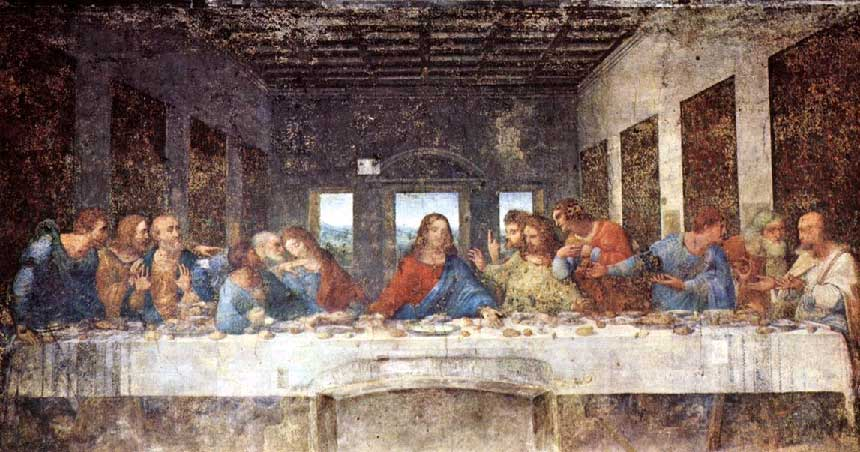
\includegraphics[angle=0,width=0.85\textwidth]{afsnit/afprovning/billeder/thressholds/medium_farver/medium_detalier/mDetalier1.jpg}
        \label{Orginal3}}
        \caption[]{Edgedetection på et billedet med medium farver og medium detalier, hvor tærskenværdigern [200,460] er den beste}
     \label{tre}
\end{figure}

\begin{table}[!h]
    \centering
    \begin{tabular}{| l | l | l | l |} \hline
        & Svage farver 	& Medium farver & Kraftige farver \\ \hline
        Få detaljer 		& (100,250)		& (100,240)		& (200,320)\\ \hline
        Medium detaljer 	& (100,280)		& (200,460)		& (200,380)\\ \hline
        Mange detaljer		& (200,400)		& (200,380)		& (300,750)\\ \hline
    \end{tabular}
    \caption{Tabel over kantdetektionstærskelværdier for ni malerier}
    \label{thressholdsTabelKant}
\end{table}

Som man kan se af tabel \ref{thressholdsTabelKant} gå tærskelværdierne
fra $(100,240)$ til $(300,750)$, så vi tager en gennemsnit af værdierne
og få at de to tærskelværdier skal være (177 og 384). 

Vi har dog i vores forsøg regnet med værdierne 78 og 194, da vores
indledende afprøvninger afviger en smugle fra den denne afprøvning.

\subsection{Afvigelsen af farver i floodfill}
Floodfill har 2 tærskelværdier $lo$ og $up$, som betegner hvor mange
pixel værdier en nabo pixel farver må variere, ned og op. En
fyldestgørelses beskrivelse af floodfill findes i afsnit
\ref{section_opdeling}. 

Vi har tænkt os at finde en fældes tærskelværdi til brug i vores
program. Måde vi gør det på at ved at observere hvordan floodfill virker
med forskellige tærskelværdier og finde de tærskelværdier som passer
bæst til maleriet. Resultatet for observationen kan ses i tabel
\ref{thressholdsTabelFF}, hvor de 9 sammen kategorier er vist og
afprøvet på de samme 9 malerier. Et af de malerierne kan se i
figur \ref{Floodfillbilledet}, hvor man kan se hvad vi har valt til at
være de optimale værdier.

\begin{figure}[!h]
    \centering
    \subfloat[8,8]{
        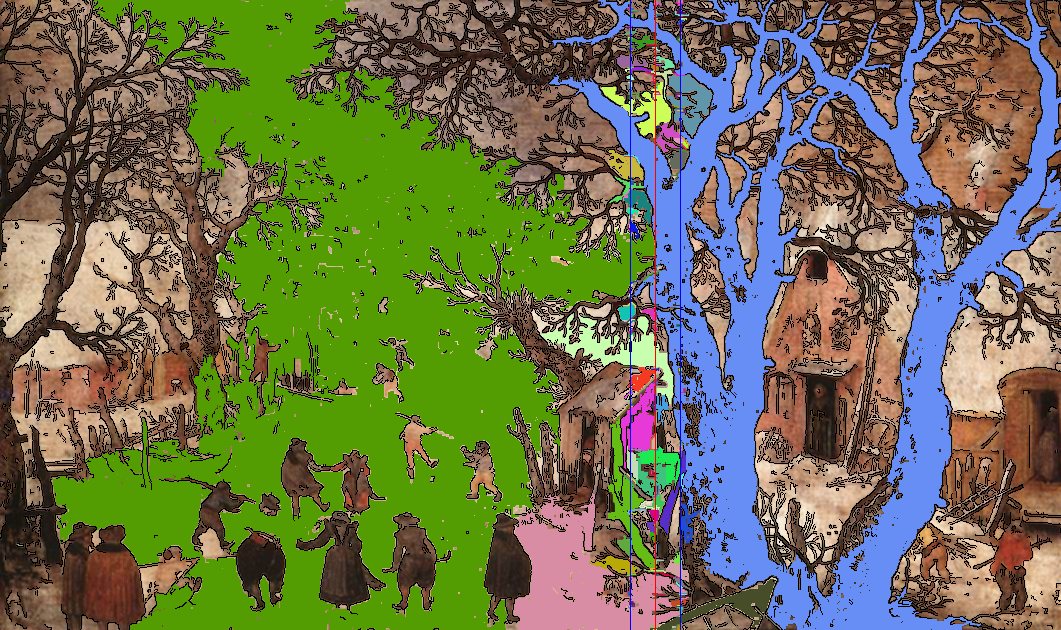
\includegraphics[angle=0,width=0.9\textwidth]{afsnit/afprovning/billeder/thressholds/svage_farver/kraftige_detalier/floodfill/8-8.png}
        \label{8-8}}\\
    \subfloat[Orgina. Navn: Winter Landscape. År: Ukent. Af:Avercamp, Hendrick.]{
        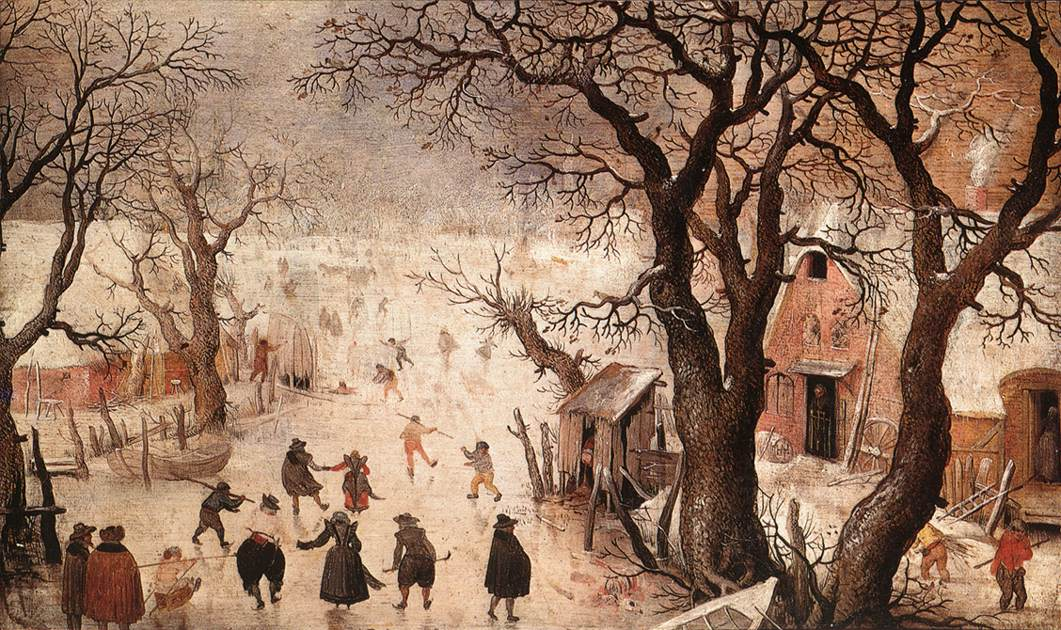
\includegraphics[angle=0,width=0.9\textwidth]{afsnit/afprovning/billeder/thressholds/svage_farver/kraftige_detalier/kDetalier.jpg}
        \label{Orginal4}}
    \caption[]{tærskelværdierne på et billedet med svage farver og kraftige detaljer hvor tærskelværdien [8,8] passer best}
    \label{Floodfillbilledet}
\end{figure}

\begin{table}[!h]
    \centering
    \begin{tabular}{| l | l | l | l |} \hline
        & Svage farver 		& Medium farver & kraftige farver \\ \hline
        Få detalier 		& \textbf{[2,2]}	& [3,3]			& [4,4]\\ \hline
        Medium detalier 	& \textbf{[2,2]}	& \textbf{[5,5]}& \textbf{[2,2]}\\ \hline
        Mange detalier		& [8,8]				& [4,4]			& [7,7]\\ \hline
    \end{tabular}
    \caption{Tabel over floodfill tærskelværdier på 9 malerier}
    \label{thressholdsTabelFF}
\end{table}

Som man kan se af tabel \ref{thressholdsTabelFF}, er nogle af vadierne
med fed, begrundelsen for det, er at vadierne, er de beste, vi kan finde
for billedet, men at de vadier stadig ikke giver noget som er særlige
brugbart. værdigerne i tabel fluktuere også en del, så vi tager
gennemsnittet og får tærskelværdierne til at være (5,5).
